\graphicspath{{Images/}}

\section{Part 3 - Forward vs Backward}

\textit{Implement and compare Repeated Forward A* and Repeated Backward A*
with respect to their runtime or, equivalently, number of expanded cells. Explain your observations in detail, that is, explain
what you observed and give a reason for the observation. Both versions of Repeated A* should break ties among cells with
the same f-value in favor of cells with larger g-values and remaining ties in an identical way, for example randomly.}

The source code contains the implementation for Repeated Backward A*. When the commented section within the main method, responsible for executing both versions across all generated mazes and computing the average time and expanded cells, is uncommented, the ensuing results are as follows.

\begin{figure}[h]
    \centering
    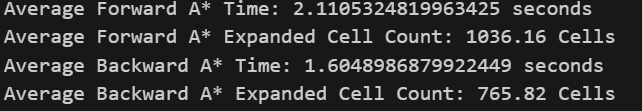
\includegraphics[width=.85\linewidth]{imgs/Results of Foward A vs Backward A.png}
    \caption{Comparison of Repeated Forward A* and Repeated Backward A*}
    \label{fig:my_label}
\end{figure}

Upon comparison of the two pathfinder algorithms, it becomes evident that the Repeated Backward A* variant exhibits superior performance. This can be attributed to a key factor: the heightened accuracy of the heuristic function when estimating distances from the goal state as opposed to the initial state. Recognizing the goal state is generally more straightforward, enhancing the reliability of the heuristic in the backward direction. Furthermore, Repeated Backward A* showcases a tendency to expand fewer nodes in contrast to Repeated Forward A*, initiating its search from the goal state and proceeding backward towards the initial state. This targeted exploration of pertinent paths leads to a diminished search space and swifter convergence toward the goal. The goal-directed approach of backward search enables the algorithm to prioritize the most promising paths, thereby contributing to a more efficient exploration process.



